
\documentclass[fleqn,12pt]{article}

\usepackage[margin=15mm]{geometry}
\usepackage[utf8]{inputenc}
\usepackage[bulgarian]{babel}
\usepackage[unicode]{hyperref}
\usepackage{amsfonts}
\usepackage{amssymb}
\usepackage{enumitem, hyperref}
\usepackage{upgreek}
\usepackage{indentfirst}
\usepackage{graphicx}
\usepackage{array}

\usepackage{amsmath}

\graphicspath{ {./img/} }

\title{Тема 15\\ Модели на разпределени софтуерни архитектури. Среди и протоколи за разпределени приложения.}

\author{v0.1}
\date{25 юни 2021}

\begin{document}

\maketitle
\tableofcontents
\pagebreak

\section{Параметри на паралелната и разпределената обработка}

\subsection{Конкурентна обработка}

\textbf{\textit{Конкурентна обработка}} наричаме обработка на данни, която се извършва от няколко процеса (нишки)
върху няколко машини (които ще наричаме възели). \textbf{Паралелната} обработка се извършва върху \textbf{една} машина,
докато \textbf{разпределената} ползва повече машини. Обикновено при паралелната обработка целта е \textbf{ускорение},
а при разпределената - \textbf{функционално разслояване}. Разбира се, ускорението също може да е (и често е) цел 
и в разпределената обработка.

\subsection{Параметри на конкуретната обработка}

\subsubsection{Паралелизъм}
\textbf{\textit{Паралелизъм}} наричаме броя процеси (нишки), които изпълняват дадена задача.
Той се дели на два типа - \textbf{софтуерен} и \textbf{хардуерен}. Софтуерният паралелизъм е 
характеристика на програмите - колко процеса (нишки) се стартирата. Хардуерният паралелизъм 
зависи от броя процесори (вкл. ядра), върху които се изпълнява задачата.
Ускорението от софтуерния паралелизъм е ограничено от хардуерния - не можем да очакваме 
8 пъти ускорение от 8 нишки, ако машината има само 2 ядра.

Обикновено паралелизмът отбелязваме с $p$.

\subsubsection{Грануларност}
\textbf{\textit{Грануларност}} е степента на декомпозиция на данните, т.е. на колко подзадания се разбива цялата задача.
Различават се три вида грануларност, като те се характеризират по ефекта си, а не по конкретни числа (защото 
числата за различни за различни задачи):
\begin{itemize}
    \item \textbf{едра} - малък брой подзадачи. В този случай малко време се прекарва в разпределение, но баланса е лош.
    \item \textbf{фина} - много голям брой подзадачи. Балансът на задачите е много добър - всеки процес получава еднакъв брой 
    \textit{операции}, но разпределянето на задачите отнема много време и забавя значително системата.
    \item \textbf{средна} - компромис между горните две. Това е грануларността, към която се стремим.
\end{itemize}

\subsubsection{Балансиране}
Както казахме, \textbf{\textit{балансирането}} се грижи всеки процес да получи еднакво количество \textit{работа}.
Това е желано, защото времето за работата на паралелен алгоритъм е времето на приключване на \textbf{най-бавния} процес (нишка).
Следователно е нежелано един процес да приключи работа, докато друг е претоварен със задания.

Балансирането можем да разделим на \textbf{статично} и \textbf{динамично}, в зависимост от това кога се случва.
Динамично балансиране е удачно (и дори наложително), когато нови задания постъпват по време на изпълнение.
Можем да разделим балансирането и по начина, по който се осъществява:
\begin{itemize}
    \item централно 
    \item разпределено (напр. верига, решетка, хиперкуб)
    \item йерархично
\end{itemize}

\subsubsection{Синхронизация}
\textbf{\textit{Синхронизацията}} описва \textbf{обмена на информация} между процесите и как той се случва.
Можем да разделим алгоритмите на три вида според нея:
\begin{itemize}
    \item \textbf{асинхронни} - не се обменят данни между процесите
    \item \textbf{локално синхронни} - всеки процес си има дефинирани съседи, с които обменя информация
    \item \textbf{глобално синхронни} - всеки процес си говори със всеки друг (пълен граф)
\end{itemize}

\subsubsection{Тип на декомпозицията}
Декомпозицията на задачата може да е по данни и по управление. В първия случай имаме \textbf{SPMD (Single Program, Multiple Data)}, а
във втория - \textbf{MPMD (Multiple Program, Multiple Data)}. Тази характеристика е ортогонална на това дали ползваме една или много машини 
- и двата типа алгоритъма могат да се прилагат на двата случая. Разликата е, че при \textbf{SPMD} ползваме една и съща програма, 
която стартираме върху различните данни. В другия случай имаме няколко различни програми.

\subsection{Метрики}
\subsubsection{Ускорение и ефикасност}
\textbf{\textit{Ускорение (acceleration)}} пресмятаме чрез $S_p = \frac{T_1}{T_p}$, където $T_1$ е времето за серийна обработка, а $T_p$ е времето за паралелна обработка при степен на паралелизъм $p$.
Поради наличие на комуникационни и синхронизационни закъснения обикновено $S_p \in (1, p)$ - ще разгледаме контрапримери след малко.

\textbf{\textit{Ефективност (efficiency)}} е нормализирано ускорние: $E_p = \frac{S_p}{p}$, като съответното обикновено стойностите са до 100\%.

\subsubsection{Суперлинейна аномалия}
Този тип аномалия настъпва, когато получим $S_p > p$. Обикновено се случва заради кеша на данните.
При пускане на повече нишки може да се включат повече хардуерни ядра, като всяко от тях има собствен \textbf{L1} кеш.
Допълнително, ако областите от данни се припокриват между нишки, то дадено парче данни се зарежда само веднъж от 
бавната оперативна памет, и след това се достъпва бързо от споделеният \textbf{L2} кеш.

\subsubsection{Нелинейна аномалия}
Това се случва когато получим $S_{p+1} < S_p$ за някое $p$, т.е. програмата се забавя при увеличаване на паралелизма.
Причините за това може да са алгоритмични, или просто сме надвишили хардуерния паралелизъм, зареди което трупаме единствено
време за \textbf{context switching}, балансиране и разпределяне, но работата не се върши по-бързо.

\subsubsection{Графика на ускорението и ефикасността}
Обикновено за дадена система се рисуват фамилия криви ускорение (и/или ефикасност), в зависимост от някой неин параметър.
Най-често този параметър е гранулярността. Ще покажем примерни графики, които включват и двете аномалии.

\begin{center}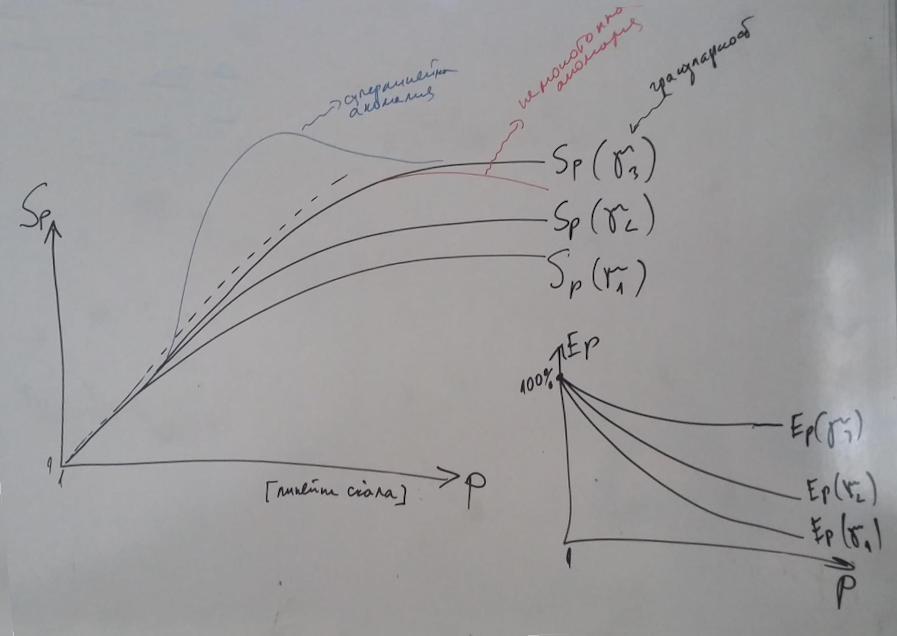
\includegraphics[width=180mm]{speedup_efficiency.png}\end{center}

\subsubsection{Закон на Амдал}
Всеки алгоритъм се състои от серийна част и част, която може да бъде паралелна. Това налага горна границата на 
възможното ускорение, която се изразява чрез \textbf{закона на Амдал}:
\[ S_{latency}(s) = \frac{1}{(1-p) + \frac{p}{s}} \]
където:
\begin{itemize}
    \item $S_{latency}$ е теоретичното ускорение на изпълнението на цялата задача.
    \item $s$ е ускорението на секцията, която паралелизираме.
    \item $p$ е фракцията от времето на задачата заемано от секцията, която сме паралелизирали, при серийно изпълнение на алгоритъма.
\end{itemize}

\subsection{Сравнение между паралелна и разпределена обработка}
\begin{center}
    \begin{tabular}{ | m{60mm} | m{60mm}| m{60mm} | } 
    \hline
    \textbf{Параметър / Тип обработка} & \textbf{Паралелна} & \textbf{Разпределена} \\ 
    \hline
    \textbf{Инфраструктура} & мултипроцесор & мултикомпютър \\ 
    \hline
    \textbf{Обмен на данни} & Обща памет и механизми за синхронизация & Предаване на съобщения чрез \textbf{middleware} \\ 
    \hline
    \textbf{Обичайна декомпозиция} & \textbf{SPMD} & \textbf{MPMD} \\ 
    \hline
    \textbf{Примери за синхронни задачи} & nBody, WaTor & Client-server, P2P, някои конвейери \\ 
    \hline
    \textbf{Примери за асинхронни задачи} & фрактали & някои конвейери \\ 
    \hline
    \end{tabular}
\end{center}

\section{Модели на разпределените софтуерни архитектури и техните структури, организация, компоненти и приложение}

\subsection{[НЕ ЗАДЪЛБАВАЙ] Дефиници}
\textbf{\textit{Софтуерната архитектура}} дефинира какви са съставните процеси на една софтуерна система, как те са структурирани и си взаимодействат.
\textbf{\textit{Моделите на софтуерни архитектури}} представляват богати на информация и точни диаграми, описващи дизайна на системата.
Под дизайн се разбира съвкупността от декомпозицията на съставните компоненти, техните функции, прилагания архитектурен стил и качествени атрибути.

\subsection{[НЕ ЗАДЪЛБАВАЙ] Процедурни модели}

\textbf{\textit{Процедурните архитектурни модели}} се базират на разпределена обработка чрез \textit{отдалечено извикване на процедури (remote procedure call (\textbf{RPC}))} или \textit{Remote Method Invocation (\textbf{RMI})}.
Представлява извикване на процедура на един възел от друг възел, като това това е прозрачно за извикващия възел, т.е. е като локална за него процедура.

\subsection{[НЕ ЗАДЪЛБАВАЙ] Обектни модели}

\textbf{\textit{Обектно-ориентираните архитектурни модели}} се основават на разделянето на отговорностите на системата в индивидуални повторно използваеми и независими обекти, които си сътрудничат.
Основните принципи на тези модели са:
\begin{itemize}
    \item \textit{Абстракция} - опростяването на решението на реален проблем чрез дефиниране на подходящи класове.
    \item \textit{Композиция} - изграждането на обекти от други обекти.
    \item \textit{Наследственост} - автоматичното присвояване на функционалностите на едни обекти на други обекти и тяхното разширение и промяна.
    \item \textit{Капсулация} - скриването на ненужните за потребителя детайли на някои обекти.
    \item \textit{Полиморфизъм} - присвояването на едно и също име на различни операции на клас или йерархия от класове.
\end{itemize}

\subsection{Потокови модели}

\textbf{\textit{Потоковите архитектурни модели}} разглеждат системата като последователност от трансформации на последователен набор от данни.
Всеки компонент трансформира входните си данни в изходни.
Топологията на пренос на данните между тях се задава експлицитно чрез \textbf{блок-диаграми}.
Модулите поддържат \textbf{само} интерфейс по данни, но не и контролен, като те не се адресират директно, а чрез предаваните данни.

\subsubsection{Видове}
Можем да разграничим няколко вида потокови архитектури в зависимост от това кога и как се извършва обработката на данните от всеки модул:
\begin{itemize}
    \item \textit{Пакетна обработка (Batch Sequential)} - Модулите се извикват в последователен ред един след друг, като изходът от един модул се предава като вход на следващия.
    Пакетите от данните, които се обработват от всеки модул, са записани под формата на \textbf{временни файлове}, които служат за комуникация между два последователни в изпълнението си модули. 
    Ключовото е, че обработката от следващия модул може да \textbf{отложена във времето}.
    Най-често този модел се използва за асинхронна обработка на данни, като се цели оптимално използване на ресурси за сметка на паралелизъм и интерактивност.
    \textbf{Примери: } профилактика на системата; безплатна обрабтока, която се случва само когато системата не е натоварена от платени потребители.
    \begin{center} 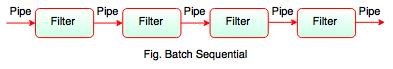
\includegraphics[width=300px]{batch_sequential.jpg} \end{center}
    \item \textit{Филтрирани канали (Pipe and Filter)} - Обработката се случва в онлайн режим. Всеки процес (отговарящ на модул) е активен
    и е свързан директно със съседите си. Всеки процес започва да предава изходните данни към следващия филтър преди да е свършил с обработката на всичките данни.
    Този начин за обработка на данни позволява паралелизъм (конвейеризация).
    \begin{center} 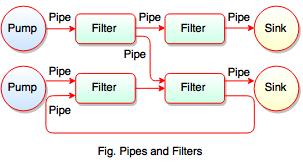
\includegraphics[width=220px]{pipe_and_filter.jpg} \end{center}
    \item \textit{Контролни процеси (Process Control)} - като \textit{Pipe and Filter}, но с добавени ограничения върху времето за изпълнение (\textbf{realtime constrainsts}).
    Понякога между модулите се добавя и пряк физически интерфейс. Както при всяка система в реално време, целта е да се гарантира време за изпълнение.
    \textbf{Примери: } управление на физически процеси, например при автомобилите и самолетите.
\end{itemize}

\subsection{Контекстни (Data centric) модели}

\textbf{\textit{Контекстните архитектурни модели}} се характеризират с централизирано хранилище за данните, от където те са достъпни за всички останали компоненти на системата.
Декомпозицията на модулите се състои от модул за \textbf{управление на достъпа до данните} и \textbf{агенти}, които извършват операции върху тях.

Интерфейсът между агентите и данните може да бъде явен (при \textbf{RMI} и \textbf{RPC}) или имплицитен (напр. \textbf{транзактивен}).
В оригинал не се предвижда комуникация между агентите.

\subsubsection{Типове}
Съществуват два основни контекстни модела:
\begin{itemize}
    \item \textit{Хранилище (Repository)}, където \textbf{агентите} са активни, т.е. те инициарат взаимодействието. Примери са СУБД, CORBA и UDDI.
    \item \textit{Черна дъска (Blackboard)}, където инициативата е на \textbf{модула с данните}, а агентите се абонати за събития (\textit{event listeners}).
    Събитие настъпва при промяна в данните.
    Използват се при AI и мултидисциплинарните системи.
\end{itemize}

\subsection{Йерархични модели}

\textbf{\textit{Йерархичните архитектурни модели}} декомпозират системата на йерархични модули, като функциите се групират по йерархичен принцип на няколко нива.
Координацията обикновено е между модули от различни нива (вертикална свързаност) и се базира на явни (т.е. "заявка-отговор") обръщения.
Слоевете делегират своята работа на услуги от съседни по-ниски нива.
Пълна прозрачност между нивата се постига при запазване на свързващите интерфейси.

Ще разгледаме два основни типа йерархични модели
\subsubsection{Слоест модел}
При този модел, имаме последователност от слоеве, като всеки предоставя услуги на по-долните.
Използван при много ОС като Unix, GNU и Windows. Също така протоколните стекове OSI и TCP/IP са слоести архитектури.
Целта на този тип архтектури е \textbf{бързо проектиране на (преносими) приложения}.

\subsubsection{Master/Slaves}
\textbf{\textit{Master/Slaves}} представлява разбиване на главна програма и подиченени програми.
Главната нарежда на подчинените какво да правят. Този модел може да цели две неща:
\begin{itemize}
    \item \textbf{отказоустойчивост и надеждност:} постига се, като главната програма проверява резултата от робите, както и статуса им
    \item \textbf{ускорение:} постига се чрез балансиране на натоварването между робите за по-ускорено изпълнение
\end{itemize}


\begin{center} 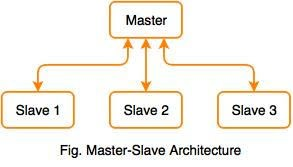
\includegraphics[width=220px]{master_slave.jpg} \end{center}

\subsection{Асинхронни модели}

\textbf{\textit{Асинхронните модели}} се базират на имплиситни асинхронни обръщения между обслужващите процеси,
т.е. обмяна на съобщения - \textbf{message passing}.

\subsubsection{Producer/Consumer}
Асинхронният обмен може да бъде от тип \textbf{Producer/Consumer}, където обменът на данни е 1:1.
Има следните разновидности:
\begin{itemize}
    \item \textit{интерактивeн (online)}, където няма буфериране и и двата процеса са активни.
    Често се ползва \textbf{адресна книга}, която позволява процесите да се адресират по име, 
    а не да трябва да знаят своя мрежови адрес - например \textbf{DNS}. 
    \item \textit{отложен (offline)}, където обмена на съобщенията се опростява посредством \textbf{процес-буфер},
    който служи като пощенска кутия. 
    Това позволява консуматора да не е активен по време на изпращане на съобщения, както и обратното.
\end{itemize}

\subsubsection{Publisher/Subscriber}
\textbf{Publisher/Subscriber} също е вид асинхронен обмен на съобщения където обменът на данни е 1:*.
Има следните разновидности:
\begin{itemize}
    \item \textit{topic-based}, където съобщенията се изпращат до topic-и, които са именувани канали.
    Издателят е отговорен за дефинирането на topic-ите, а абонатите получават съобщенията от всички topic-и, за които са се абонирали.
    \item \textbf{[Не е споменато на консултацията]} \textit{content-based}, където съобщенията се изпращат до абонат, ако атрибутите на съдържанието отговарят на ограниченията дефинирани от абоната.
    Абонатът е отговорен за класификацията на съобщенията.
\end{itemize}

\subsection{Интерактивни модели}

\textbf{\textit{Интерактивните модели}} поддържат интензивен потребителски интерфейс.
За целта декомпозицията на системата е на 3 функционални модула:
\begin{itemize}
    \item \textit{модул за представяне (изглед)}, имплементиращ потребителския интерфейс.
    Използва се за представяне (в т.ч. графично и мултимедийно) на изходните данни и намеса на потребителите в обработката (т.е. вход за данни и контрол)
    \item \textit{модул данни}, поддържащ данновия модел заедно с базова функционалност за обработката на данните
    \item \textit{модул за управление}, който отговаря за системни комуникации, управление на процесите, инициализиране и конфигуриране на модули данни, както и управление на изгледи.
\end{itemize}

Има две категории интерактивни софтуери архитектури - \textbf{PAC (Presentation-Abstraction-Control)} и \textbf{MVC (Model-View-Controller)}, където аналогията между \textbf{P-V, A-M, C-C}.
Те се различават по начина на управление като:
\begin{itemize}
    \item \textbf{PAC} е с йерархично (разслоено) и разпределено управление, при което системата се формира от набор коопериращи агенти на три нива - \textbf{базово ниво}, състоящо от агенти работещи върху общи данни и бизнес логика, \textbf{средно ниво}, състоящо от агенти координатори на изгледите и \textbf{ниво на изгледите} за обработка на локални данни.
    Всеки агент имплементира \textbf{P, A и C} компоненти.
    \begin{center} 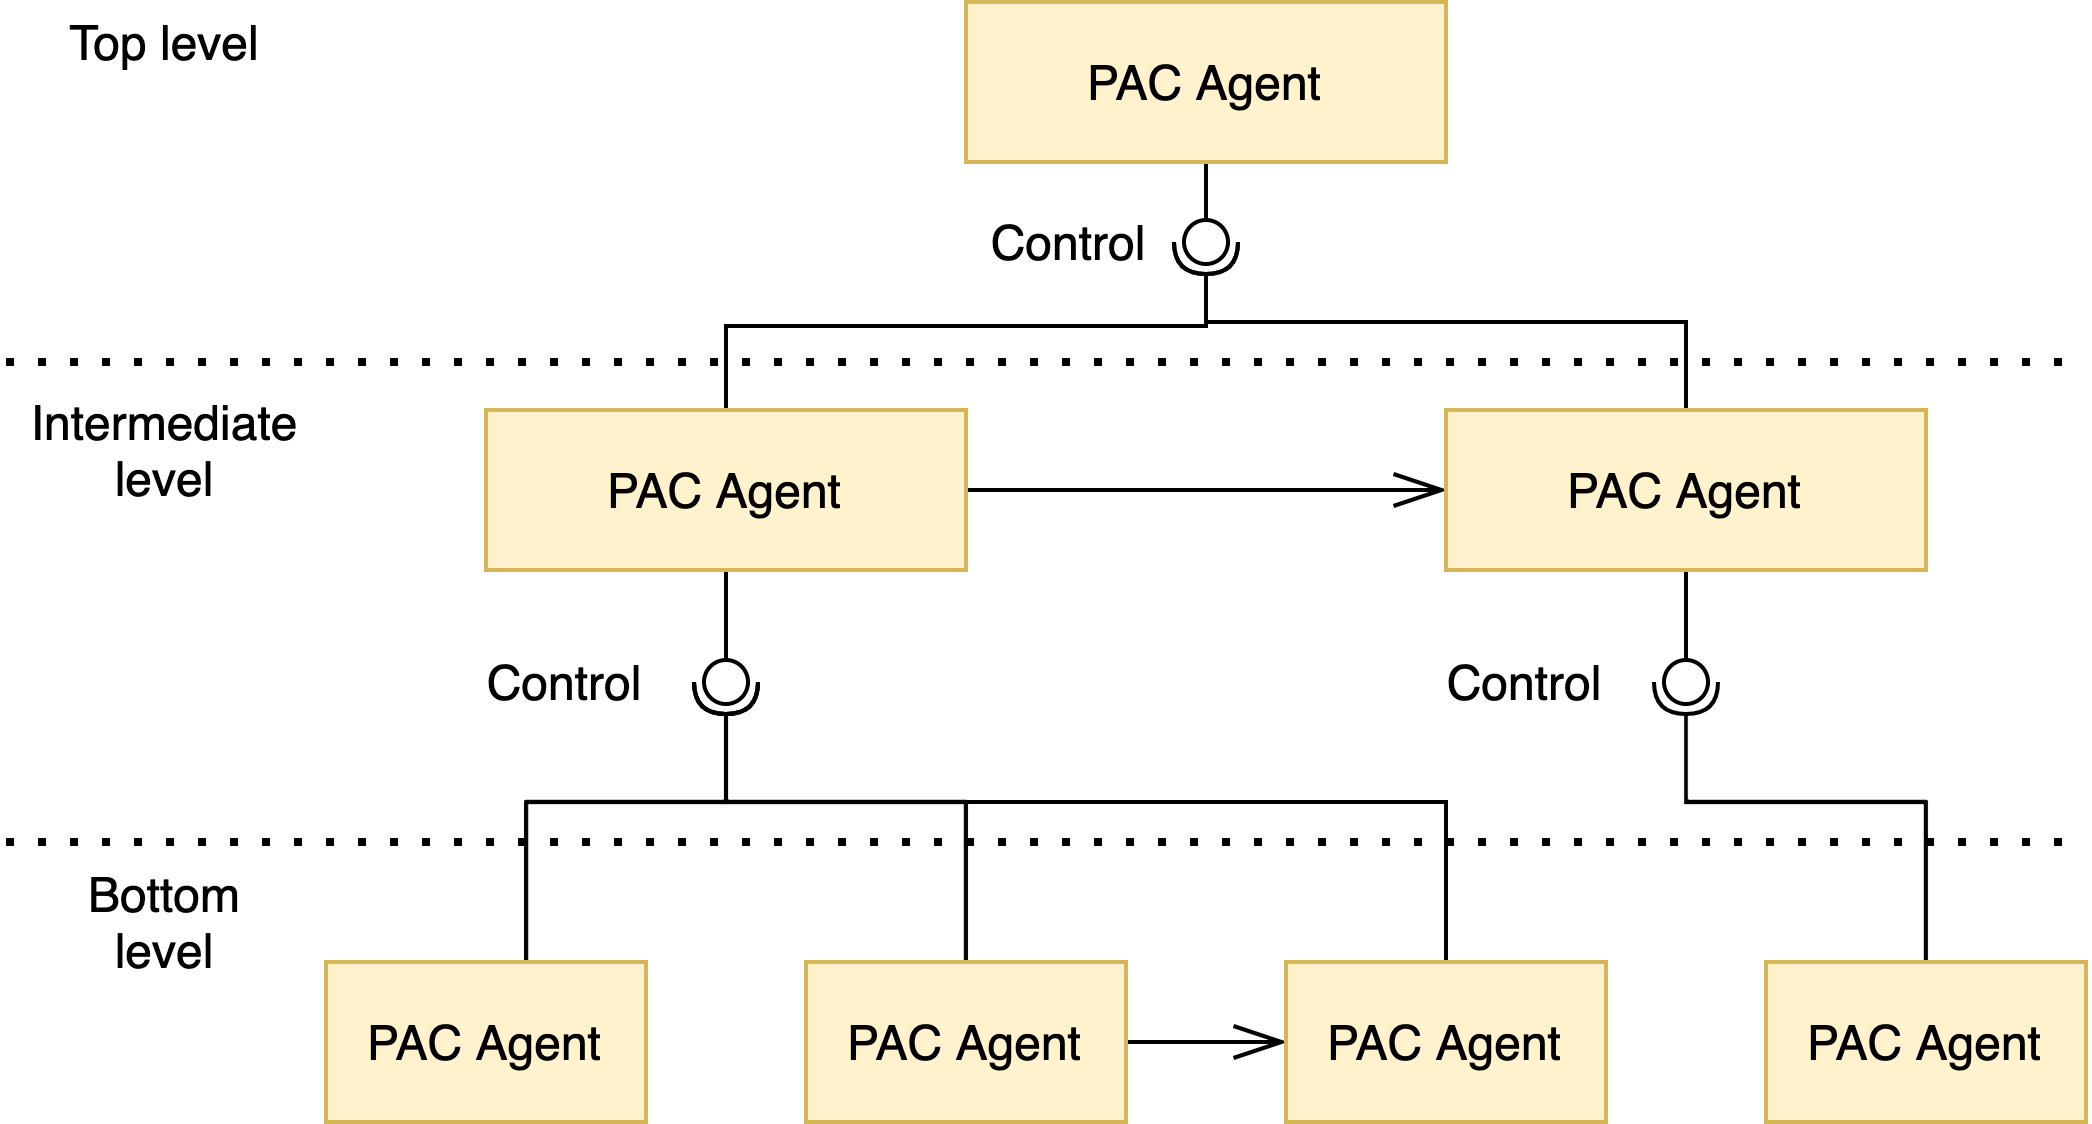
\includegraphics[width=250px]{pac.png} \end{center}
    \item при \textbf{MVC} агентите са равнопоставени.
\end{itemize}

\section{Организация на разпределените приложения}

\textbf{\textit{Multiple programs multiple data (MPMD)}} наричаме разпределени системи състоящи се от много програми паралелно извършващи работа върху различни данни.
Използват се при наличие на множество потребители, като системи за масово обслужване.

\subsection{Клиент-сървър и двуслойни архитектури}

\textbf{\textit{Клиент-сървър}} е класически \textbf{MPMD} модел за адаптиране на ограничена клиентска инфраструктура към сложни задачи.
Процесите се класифицират като два основни:
\begin{itemize}
    \item \textit{Сървър}, който е реактивен процес, имплементиращ приложната логика и данновия модел под формата на конкретен набор от услуги.
    \item \textit{Клиент}, който е активен интерфейсен процес, използващ услугите на сървъра.
\end{itemize}

Има два основни вида клиенти - \textbf{тънки (thin)}, които делегират цялата работа на сървъра, и \textbf{дебели (fat)}, които изпълняват част от задачата.
\bigbreak


\begin{center}
\begin{tabular}{ |c|c| } 
    \hline
    Предимства & Недостатъци \\
    \hline
    технологично специализиране & унификация на клиентската инфраструктура \\
    \hline
    инфраструктурна гъвкавост (скалиране) & по-трудна защита на достъпа до данните \\
    \hline
    преизползване & скалируемост на сървъра \\
    \hline
    еволюция без участието на потребителя & скъпа поддръжка, профилактика и тестване \\
    \hline
\end{tabular}
\end{center}

\subsection{N-слойни архитектури}

\textbf{\textit{N-слойната архитектура}} включва надграждане над клиент-сървър архитектурата, където компонентите са разделени на няколко слоя.
Можем да си представим, че слоевете са вертикално подредени и компонентите на даден слой са клиенти на сървъри от съседния долен слой.
\bigbreak
При \textbf{N-слойните архитектури} редовно се срещат \textbf{многослойни сървъри}, където сървърната част е декомпозирана на поне два слоя, които се класифицират като:
\begin{itemize}
    \item \textit{междинни слоеве}, които се намират между интерфейсния и вътрешния слой, имплементиращ $``$бизнес логиката$''$.
    \item \textit{вътрешен слой}, най-долният слой, който обичайно е персистентен или се използва за комуникации. 
\end{itemize}

Очевидно щом е надграждане над клиент-сървър архитектурата, то \textbf{\textit{N-слойната}} разполага със същите недостатъци и предимства, но по-силно изразени.
\bigbreak
\textbf{\textit{3-слойните архитектури}} са вид \textbf{N-слойни}, където имаме наличието на интерфейсен, междинен и вътрешен слой.

\subsection{Peer-to-Peer архитектури}

\textbf{\textit{Peer-to-Peer (P2P) архитектурата}} се разгръща като \textbf{наслоена (overlay) мрежа} върху съществуваща клиентска част от мрежова инфраструктура.
Всеки участник е еднакво привилегирован и заделя част от ресурсите си (cpu, диск и др.), която да се използва от останалите участници в мрежата без нуждата от каквато и да е централна координция.
За разлика от класическата архитектура клиент-сървър всеки участник изпълняват фукцията на клиент и сървър едновременно за другите участници.
\textbf{P2P} се характеризира чрез \textbf{децентрализирана топология}, \textbf{самоорганизация}, \textbf{инцидентна (ad hoc) и динамична свързаност и наличност} на възлите и процесите в тях, \textbf{скалируемост}, \textbf{отказоустойчивост (fault tolerance)}, анонимност на споделянето и специална юридическа регулация.

\begin{center} 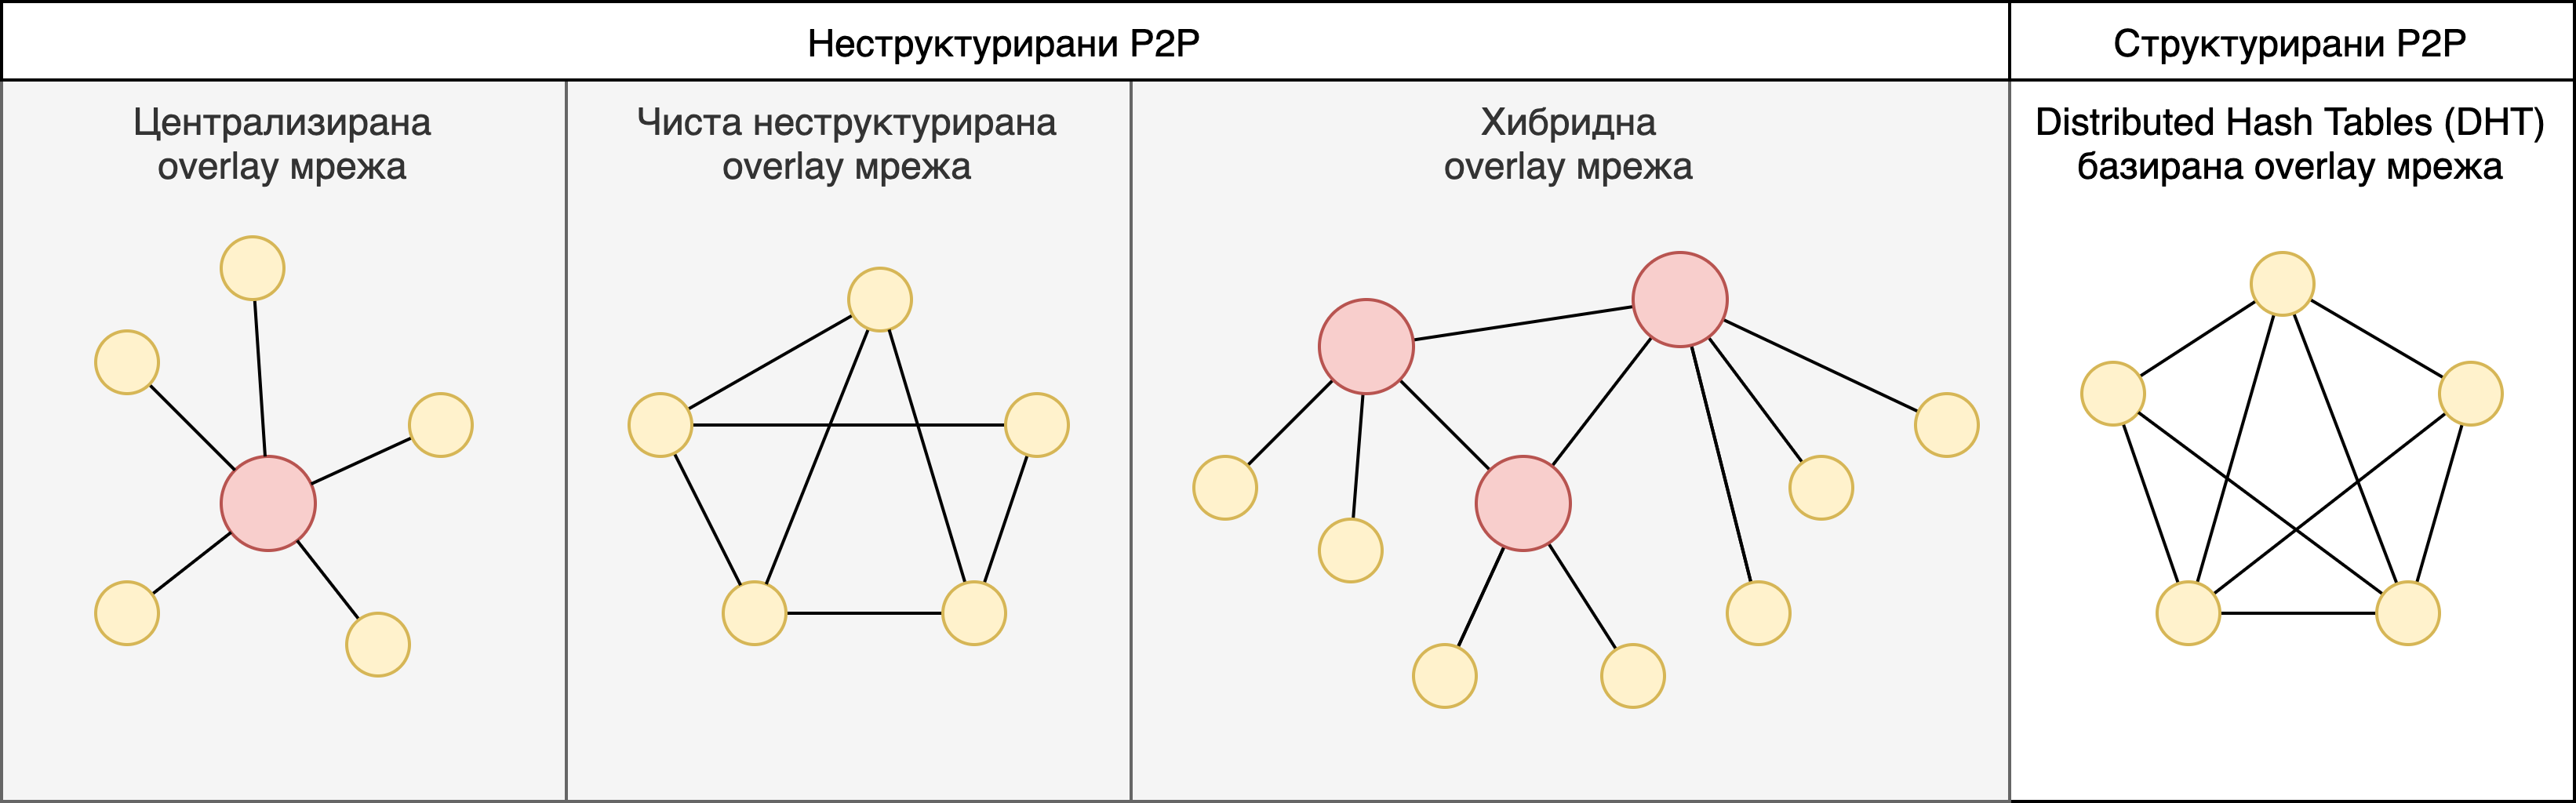
\includegraphics[width=500px]{p2p_overlay_topologies.png} \end{center}

\subsection{Сървъри за приложения и web-сървъри}

\textbf{\textit{Сървърът за приложения}} представлява съвкупност от компоненти, които могат да бъдат достъпни чрез платформено независими интерфейси за програмиране (\textbf{Application Programming Interface (API)}).
\textbf{\textit{Web-сървърите}} са вид сървъри за приложения, утилизиращи протокола \textbf{HTTP(S)}, където съдържанието, което се доставя, е основно \textbf{HTML} текст, но може да съдържа файлове дефинирани съгласно \textbf{MIME}.

\subsection{Метасистеми и грид}

Разпределените системи, могат да бъдат разделени в две категории в зависимост от свързаността и подобието на възлите си:
\begin{itemize}
    \item \textbf{клъстери} - локална мрежа от няколко хомогенни възела.
    \item \textbf{грид} - мрежа от хомогенни или хетерогенни възли, работещи заедно върху сложна задача, но разделени от големи дистаниции.
\end{itemize}

\subsection{Сервизно-ориентирани архитектури}

\textbf{\textit{Сервизно-ориентираната архитектура (Service-oriented architecture (SOA))}} е архитектурен стил където компонентите се третират като черни кутии наречени \textbf{услуги}.
\textbf{Услуга} дефинираме като самостоятелна единица, покриваща функционален домейн, която може да бъде достъпена отдалечено.
Тя може да бъде използвана посредством унифициран програмен интерфейс наречен \textbf{Application Programming Interface (API)}.

\subsection{Моделно-ориентирани архитектури}

\textbf{\textit{Моделно-ориентираната архитектура (Model-driven architecture (MDA))}} е софтуерна архитектура за автоматизирано проектиране на приложения.
Базира се на принципите на \textbf{model-driven engineering}, т.е. изграждането на абстрактни модели, които описват системата.
Целите на тази архитектура са разделянето на дизайна от конкретната имплементация.

\subsection{Аспектно-ориентирани архитектури}

\textbf{\textit{Аспектно-ориентираната архитектура}} е софтуерна архитектура, която се базира на принципите на \textbf{аспектно-ориентираното програмиране}.
При декомпозиция на модулите се появяват някои изисквания, които не могат да бъдат адекватно обособени в отделни компоненти.
Такива изисквания наричаме аспекти, като те представляват функционалности споделени между няколко компонента.
Такива са например изисквания свързани с audit logging.
Обичайно се имплементират чрез инжектиране на код в някои функции.

\subsection{Софтуерни агенти}

Софтуерните агенти са автономни софтуерни единици, които могат да изпълняват задания по заръка на своя хост.
Те се дефинират от гледна точка на своето поведение.
Присъщи техни характеристики са:
\begin{itemize}
    \item \textit{персистентност} - изпълняват се постоянно като демони и сами преценяват кога да предприемат действия.
    \item \textit{автономност} - могат да извършват задачи самостоятелно.
    \item \textit{социалност} - могат да взаимодействат с други компоненти чрез комуникация.
    \item \textit{реактивност} - агентите възприемат контекста, в който оперират и реагират спрямо него.
\end{itemize}

\end{document}
